\chapter{Výstupy datové analýzy}
\label{appendix:data-analysis-output}
V této příloze jsou zahrnuty výstupy datové analýzy jako jsou formáty jednotlivých datových sad a grafy, které se snaží zmapovat stav jednotlivých datových sad a vztahy mezi nimi.
\section{Formáty datových sad}
\begin{lstlisting}[language=json, caption=Formát datové sady Dominika Popa]
{
  "url": string,
  "puvodce": string,
  "signatura": string,
  "invCislo": string,
  "typ": string,
  "jazyk": string,
  "rozsah": string,
  "invCislo": string,
  "obsah": string[],
  "uzemi": {
    [nazev_obce]: {
      "typ": decimal,
      "ruian": decimal,
      "latitude": float,
      "longitude": float,
      "obec": string,
      "okres": string,
      "varianty": string[] 
    },
    ...
  },
  "okresy": string[]
}
\end{lstlisting}

\newpage
\begin{lstlisting}[language=json, caption=Formát datové sady Jakuba Sokolíka]
{
  "id_registra": string,
  "signature": string,
  "inv_id": string,
  "type": string,
  "scan_count": string,
  "archive": string,
  "fond": string,
  "obec": string,
  "obec_ruian": string,
  "cast_obce": string,
  "cast_obce_ruian": string
}
\end{lstlisting}

\newpage
\begin{lstlisting}[language=json, caption=Formát datové sady Jana Valuška]
{
  "type_of_record": string,
  "archive": string,
  "languages": string[],
  "signature": string,
  "inventory_number": string,
  "originator_name": string,
  "originator_type": string,
  "originator_note": string,
  "signature": string,
  "y_deceased_from": number,
  "y_deceased_to": number,
  "covered_area": [
    {
      "country": string,
      "region": string,
      "district": string,
      "municipality": string,
      "borough": string,
      "german_name": string,
      "alternative_names": string[],
    }
  ],
  "number_of_scans": number,
  "register_note": string,
  "link": string,
  "content": string,
  "other_note": string,
  "y_born_from": string,
  "y_born_to": string,
  "y_index_born_from": string,
  "y_index_born_to": string,
  "y_married_from": string,
  "y_married_to": string,
  "y_index_married_from": string,
  "y_index_married_to": string,
  "y_deceased_from": string,
  "y_deceased_to": string,
  "y_index_deceased_from": string,
  "y_index_deceased_to": string,
  "content": string,
  "description": string,
  "fund": string,
  "index_only": string,
  "judicial_district": string,
  "land_registry_nrs": string,
  "nad": string,
  "name": string,
  "original_name": string,
  "persons_counted": string,
  "record_method": string,
  "register_note": string,
  "specific_type": string,
  "y_from": string,
  "y_taken": string,
  "y_to": string,
}
\end{lstlisting}

\newpage
\begin{lstlisting}[language=json, caption=Formát datové sady se skeny]
{
  "id": string,
  "signatura": string,
  "inv. cislo": string,
  "puvodce": string,
  "misto_ulozeni": string,
  "obsah": {
    "Narození": {
        "od":  string,
        "do": string
    },
    "INDEX Narozených": {
        "od": string,
        "do": string
    },
    "Oddaní": {
        "od": string,
        "do": string
    },
    "INDEX Oddaných": {
        "od": string,
        "do": string
    },
    "Zemřelí": {
        "od": string,
        "do": string
    },
    "INDEX Zemřelých": {
        "od": string,
        "do": string
    },
    "poznamka":string
  },
  "obce_seznam": string[], //In some files of dataset just string
  "obce": [{ //In some files of dataset just string[] or string[][]
    "od": string,
    "do": string,
    "umisteni": {
        "stat": string,
        "kraj": string,
        "okres": string,
        "obec": string,
        "cast_obce": string,
        "samota": string
    }
  }],
  "jazyky": string[],
  "snimky": {
    "jmeno": string,
    "url": string[]
  }
}
\end{lstlisting}



\section{Grafy pro jednotlivé archivy}

\noindent\textbf{Moravský zemský archiv}\\
\begin{figure}[htbp]
\centering
    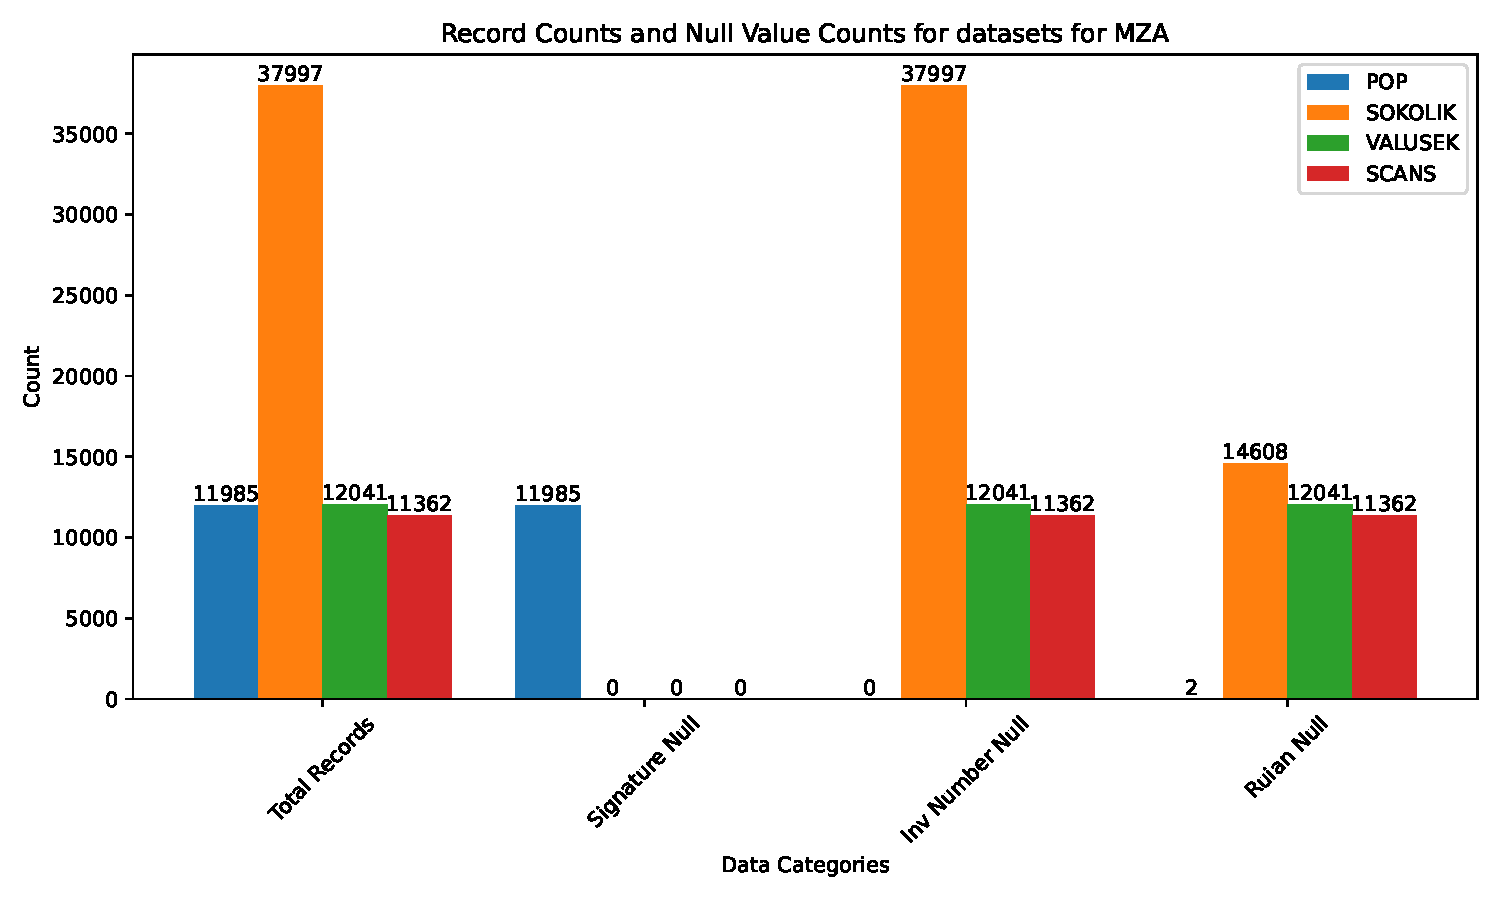
\includegraphics[scale=.5]{obrazky-figures/dataAnalysis/mza/missingValues.pdf}
    \caption{Analýza chybějících hodnot pro MZA}
\end{figure}

\begin{figure}[htbp]
\centering
    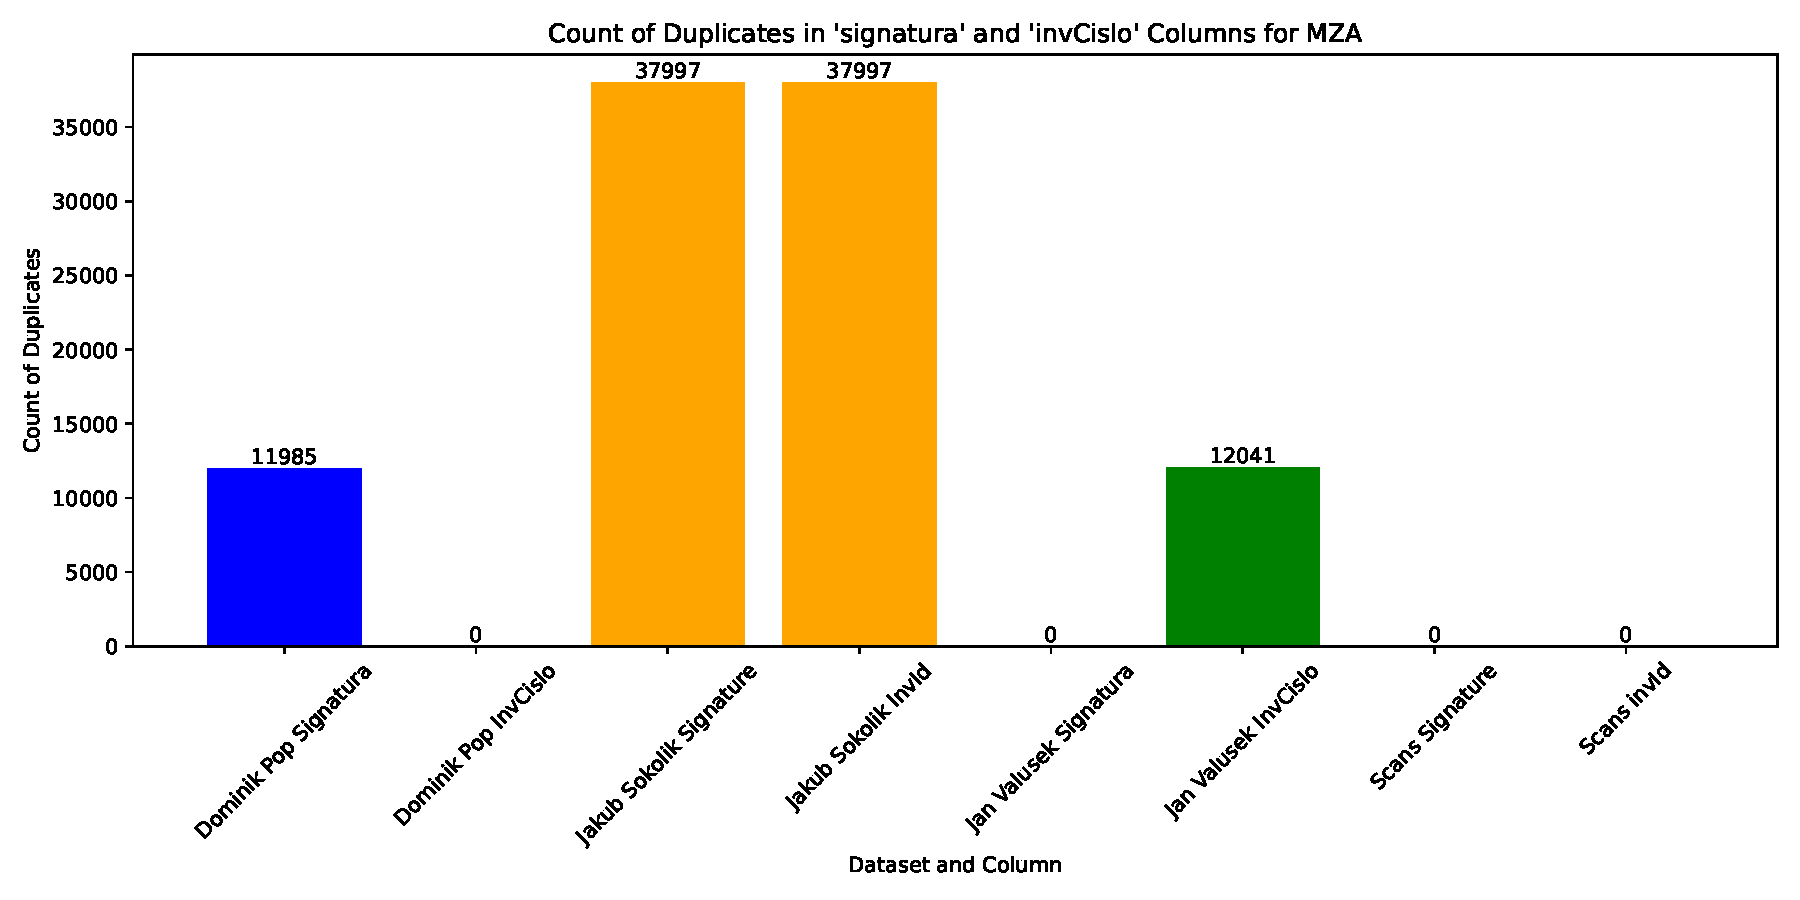
\includegraphics[scale=.5]{obrazky-figures/dataAnalysis/mza/duplicities.pdf}
    \caption{Analýza duplicitních hodnot pro MZA}
\end{figure}

\begin{figure}[htbp]
\centering
    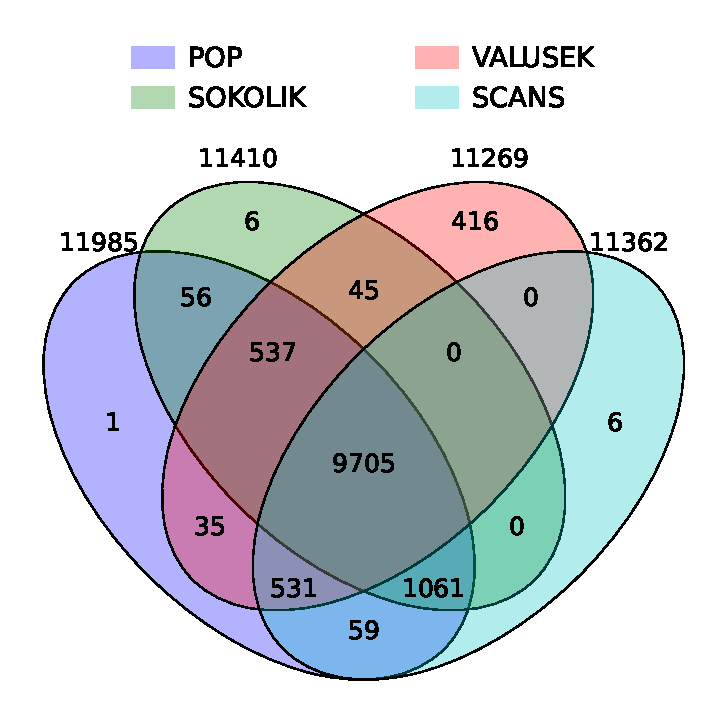
\includegraphics[scale=.5]{obrazky-figures/dataAnalysis/mza/Venn_4.pdf}
    \caption{Vennův diagram pro MZA}
\end{figure}

\begin{figure}[htbp]
\centering
    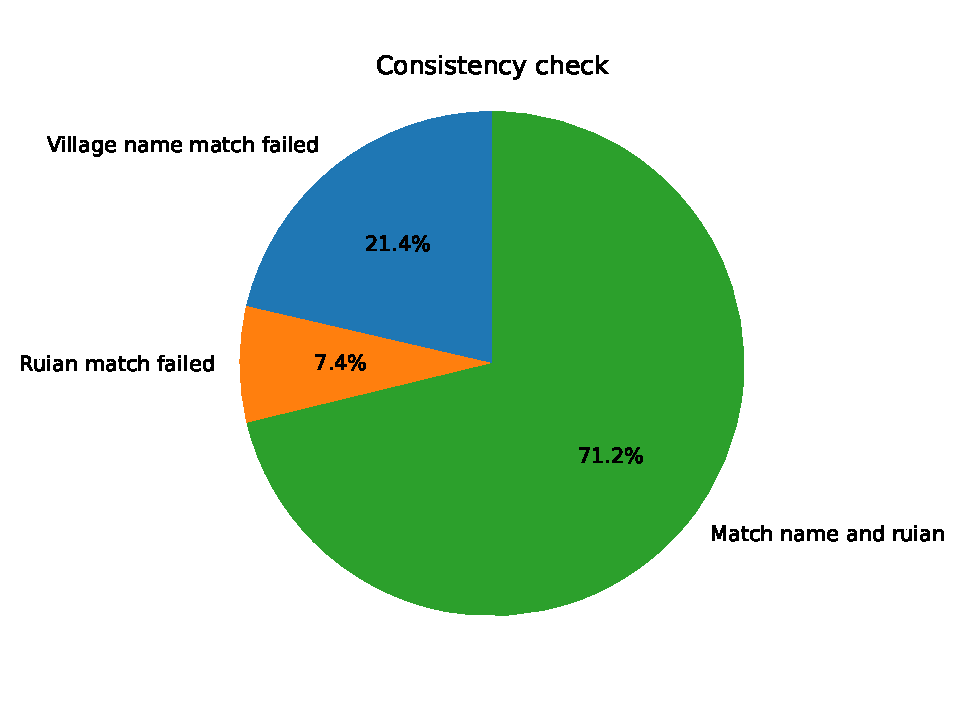
\includegraphics[scale=.7]{obrazky-figures/dataAnalysis/mza/consistencyCheck2.pdf}
    \caption{Kontrola konzistence pro MZA}
\end{figure}

\newpage
\noindent\textbf{Archiv hlavní města Praha}\\
\begin{figure}[htbp]
\centering
    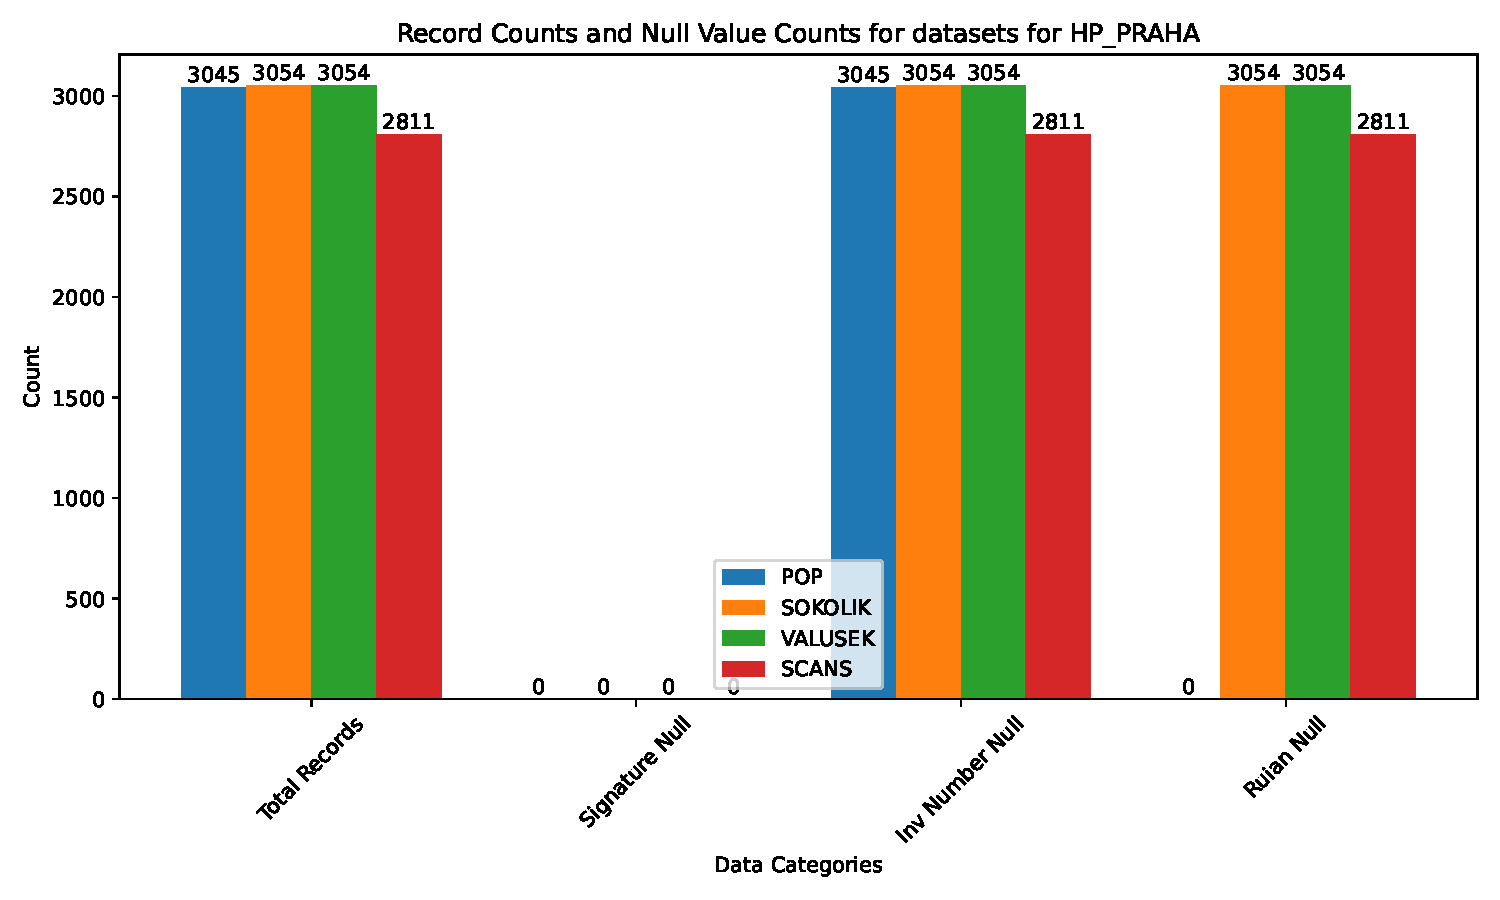
\includegraphics[scale=.5]{obrazky-figures/dataAnalysis/hpPraha/missingValues.pdf}
    \caption{Analýza chybějících hodnot pro Národní archiv}
\end{figure}

\begin{figure}[htbp]
\centering
    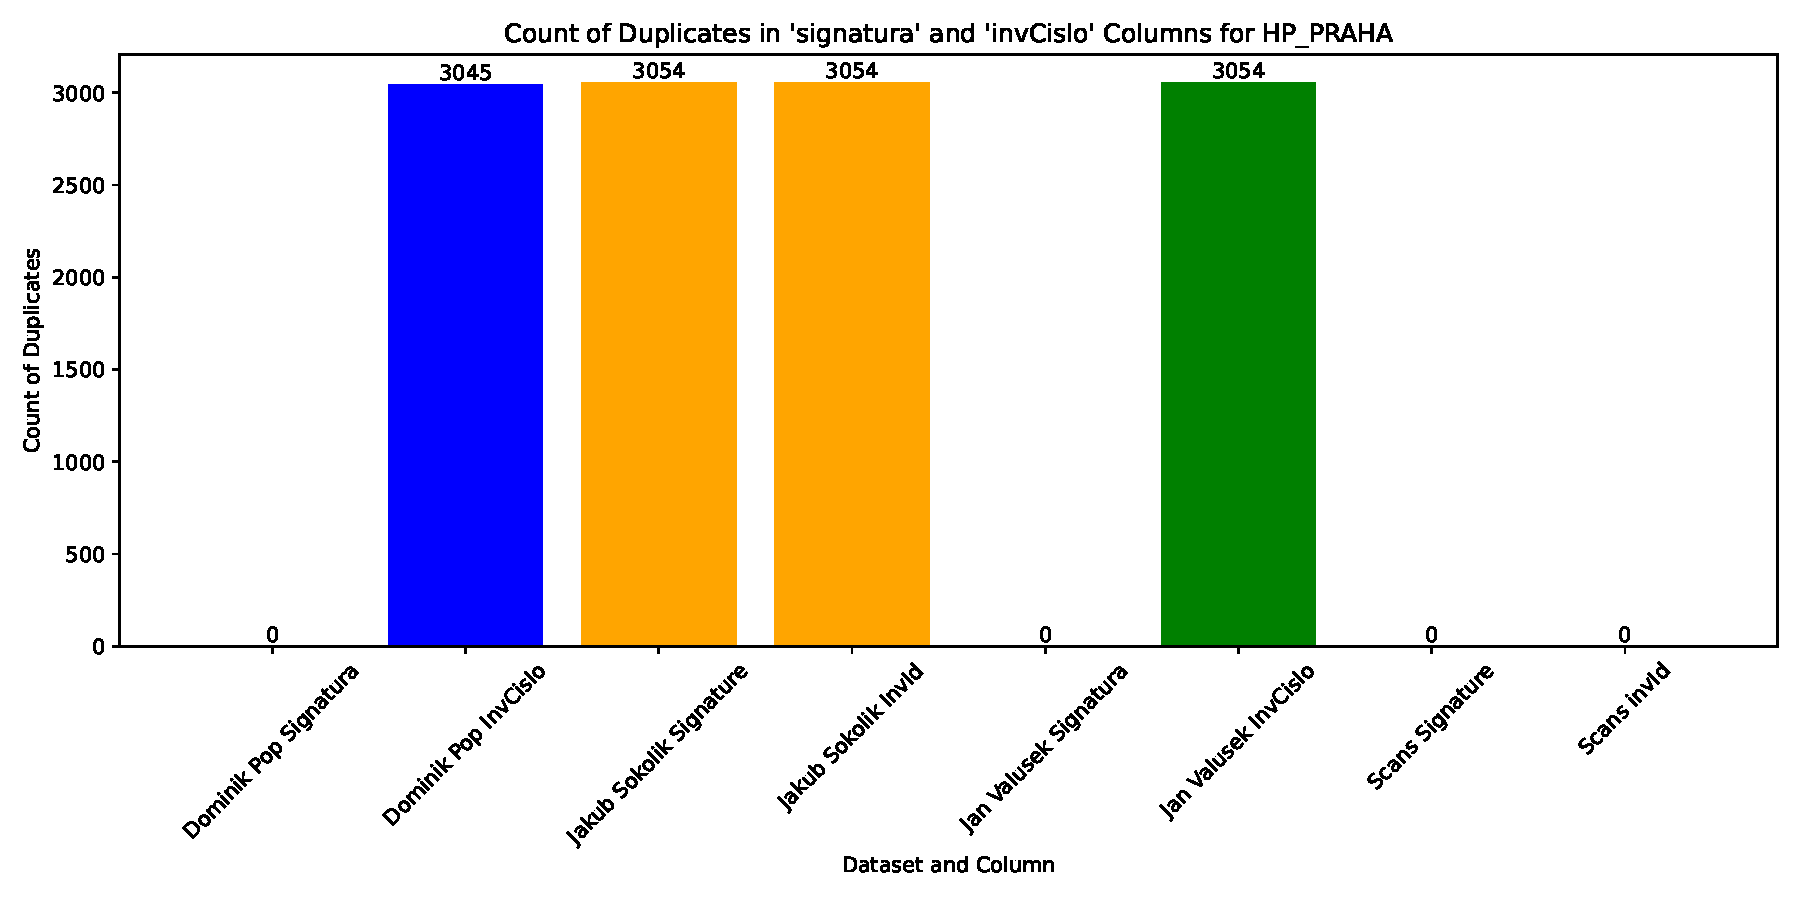
\includegraphics[scale=.5]{obrazky-figures/dataAnalysis/hpPraha/duplicities.pdf}
    \caption{Analýza duplicitních hodnot pro Národní archiv}
\end{figure}

\begin{figure}[htbp]
\centering
    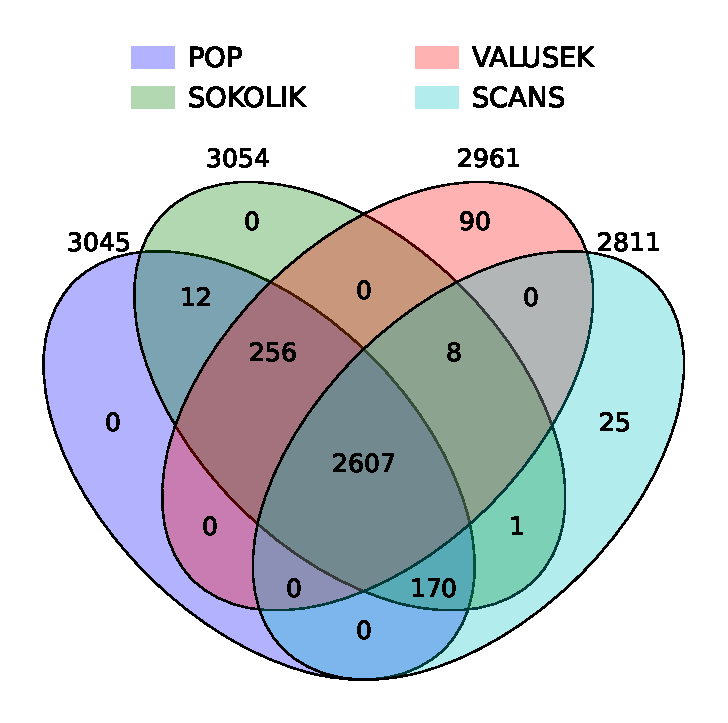
\includegraphics[scale=.35]{obrazky-figures/dataAnalysis/hpPraha/Venn_4.pdf}
    \caption{Kontrola konzistence pro Národní archiv}
\end{figure}


\newpage
\noindent\textbf{Státní oblastní archiv v Hradci Králové}\\
\begin{figure}[htbp]
\centering
    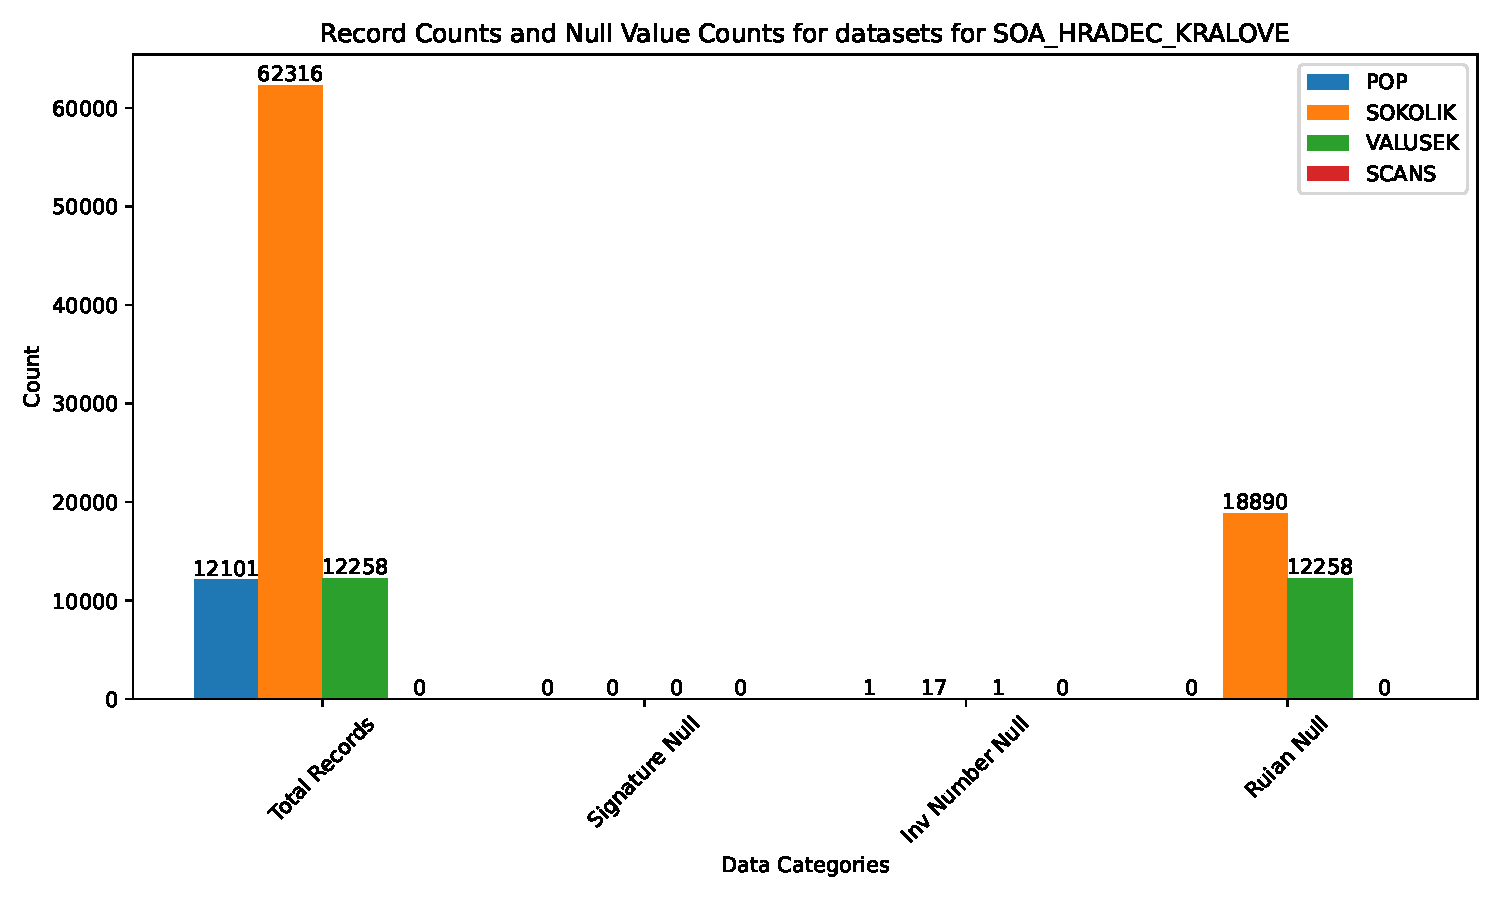
\includegraphics[scale=.5]{obrazky-figures/dataAnalysis/soaHradecKralove/missingValues.pdf}
    \caption{Analýza chybějících hodnot pro SOA v Hradci Králové}
\end{figure}

\begin{figure}[htbp]
\centering
    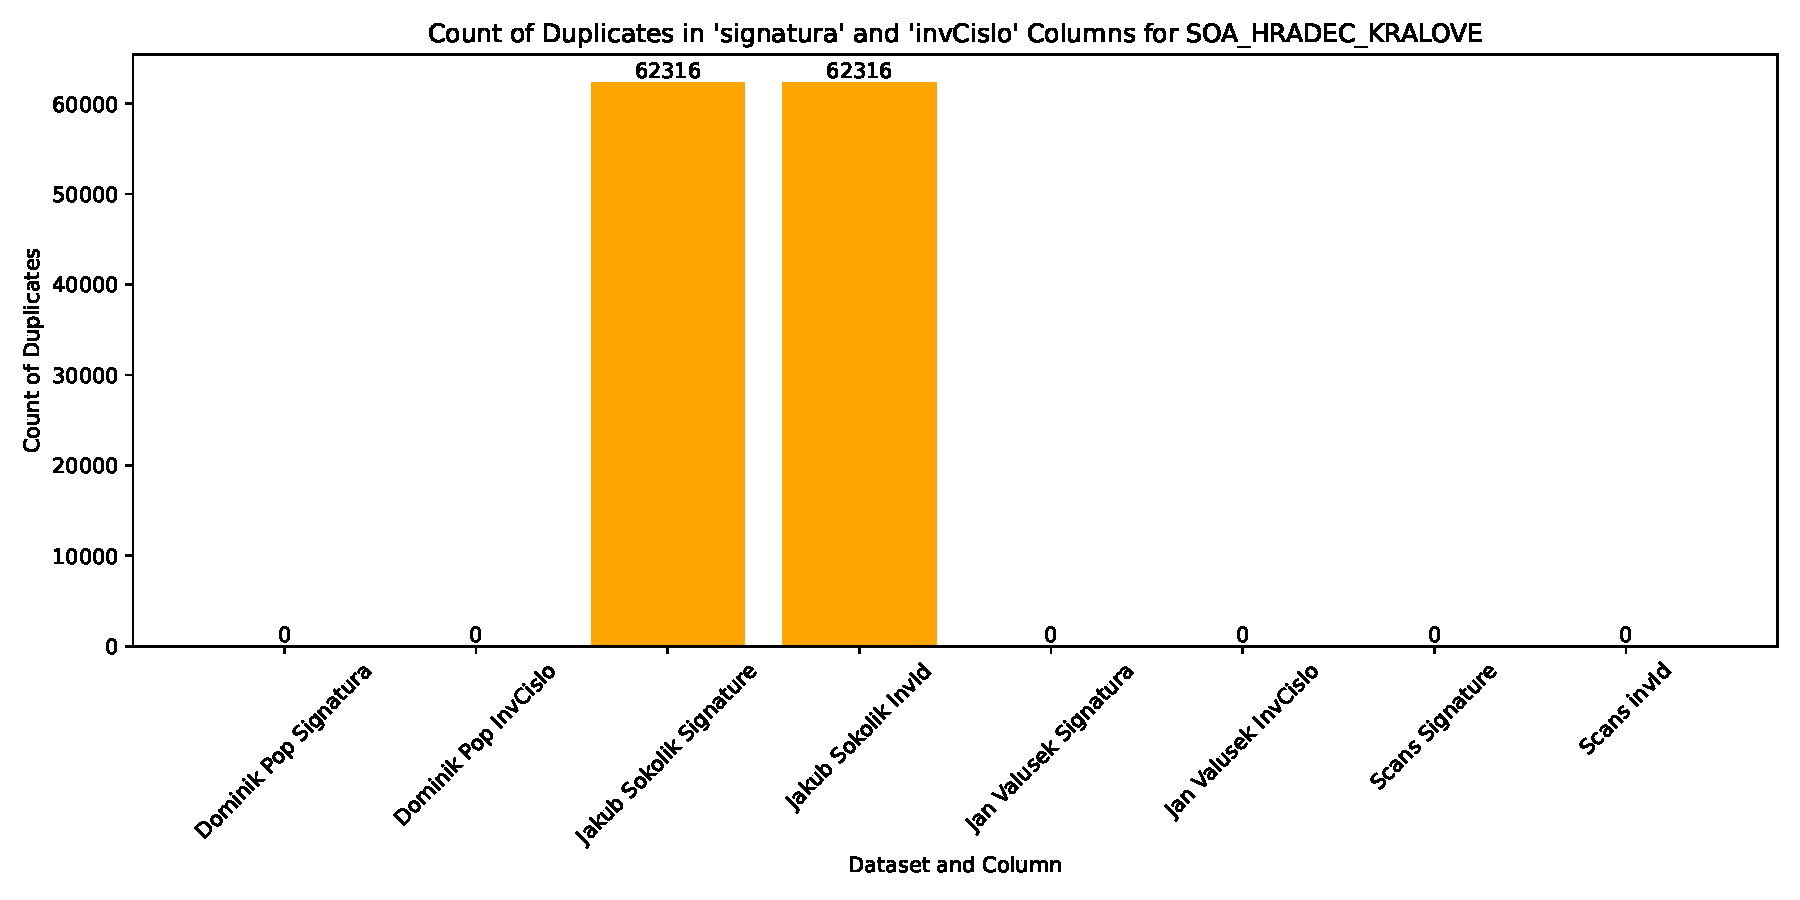
\includegraphics[scale=.5]{obrazky-figures/dataAnalysis/soaHradecKralove/duplicities.pdf}
    \caption{Analýza duplicitních hodnot pro SOA v Hradci Králové}
\end{figure}

\begin{figure}[htbp]
\centering
    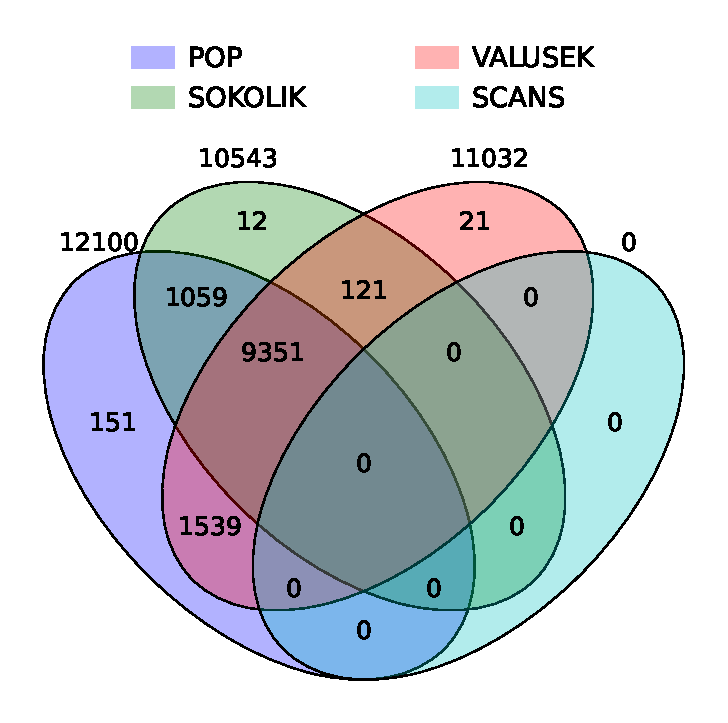
\includegraphics[scale=.5]{obrazky-figures/dataAnalysis/soaHradecKralove/Venn_4.pdf}
    \caption{Vennuv diagram pro SOA v Hradci Králové}
\end{figure}

\begin{figure}[htbp]
\centering
    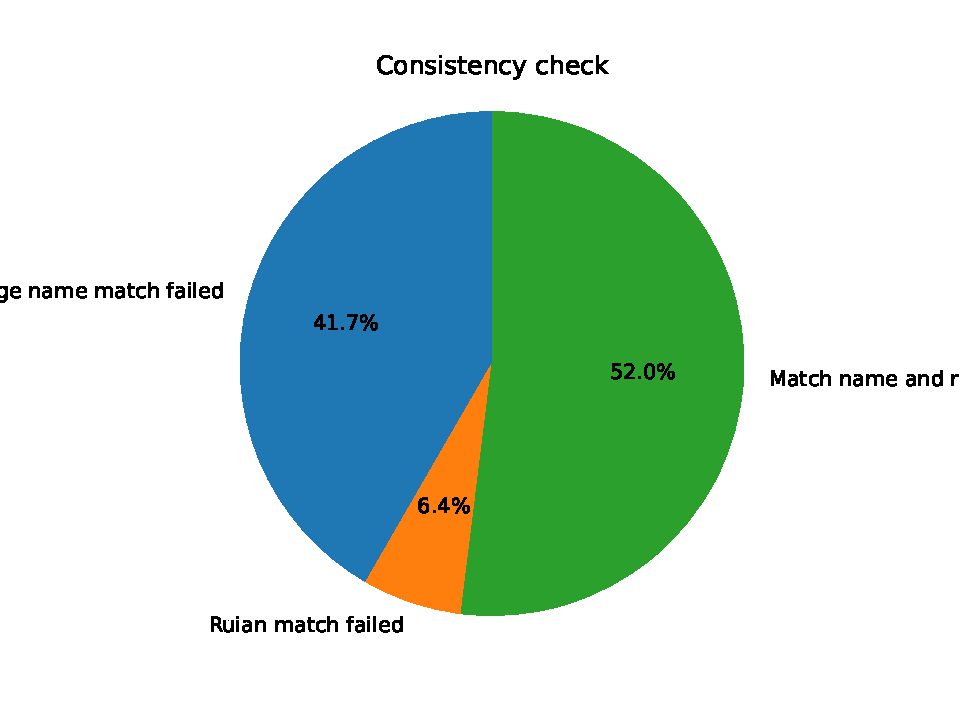
\includegraphics[scale=.5]{obrazky-figures/dataAnalysis/soaHradecKralove/consistencyCheck2.pdf}
    \caption{Kontrola konzistence pro SOA v Hradci Králové}
\end{figure}

\newpage
\noindent\textbf{Státní oblastní archiv v Litoměřicích}\\

\begin{figure}[htbp]
\centering
    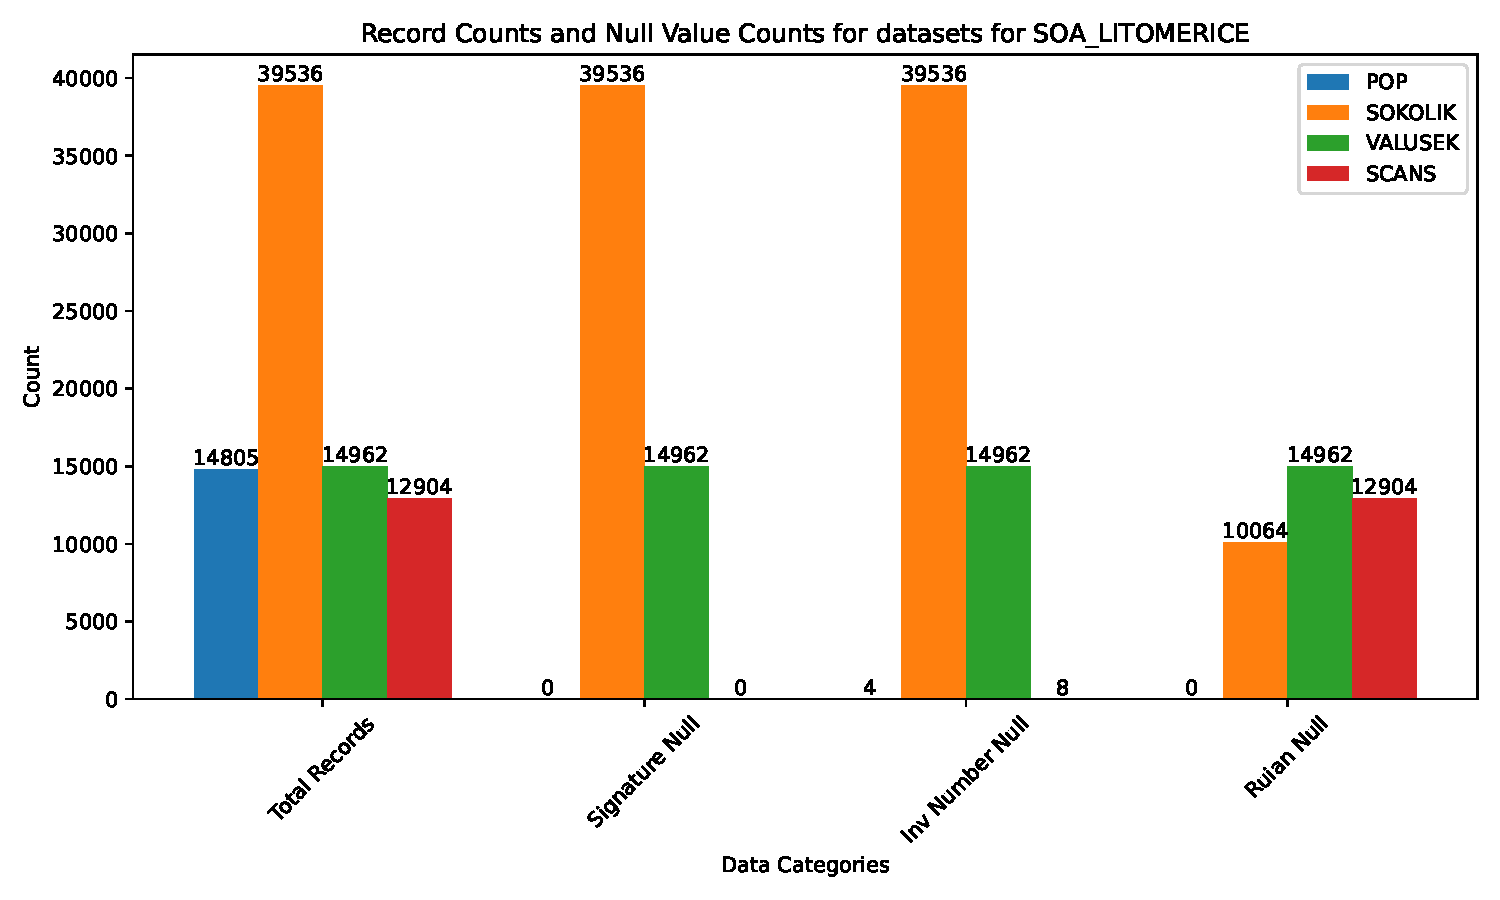
\includegraphics[scale=.5]{obrazky-figures/dataAnalysis/soaLitomerice/missingValues.pdf}
    \caption{Analýza chybějících hodnot pro SOA v Litoměřicích}
\end{figure}

\begin{figure}[htbp]
\centering
    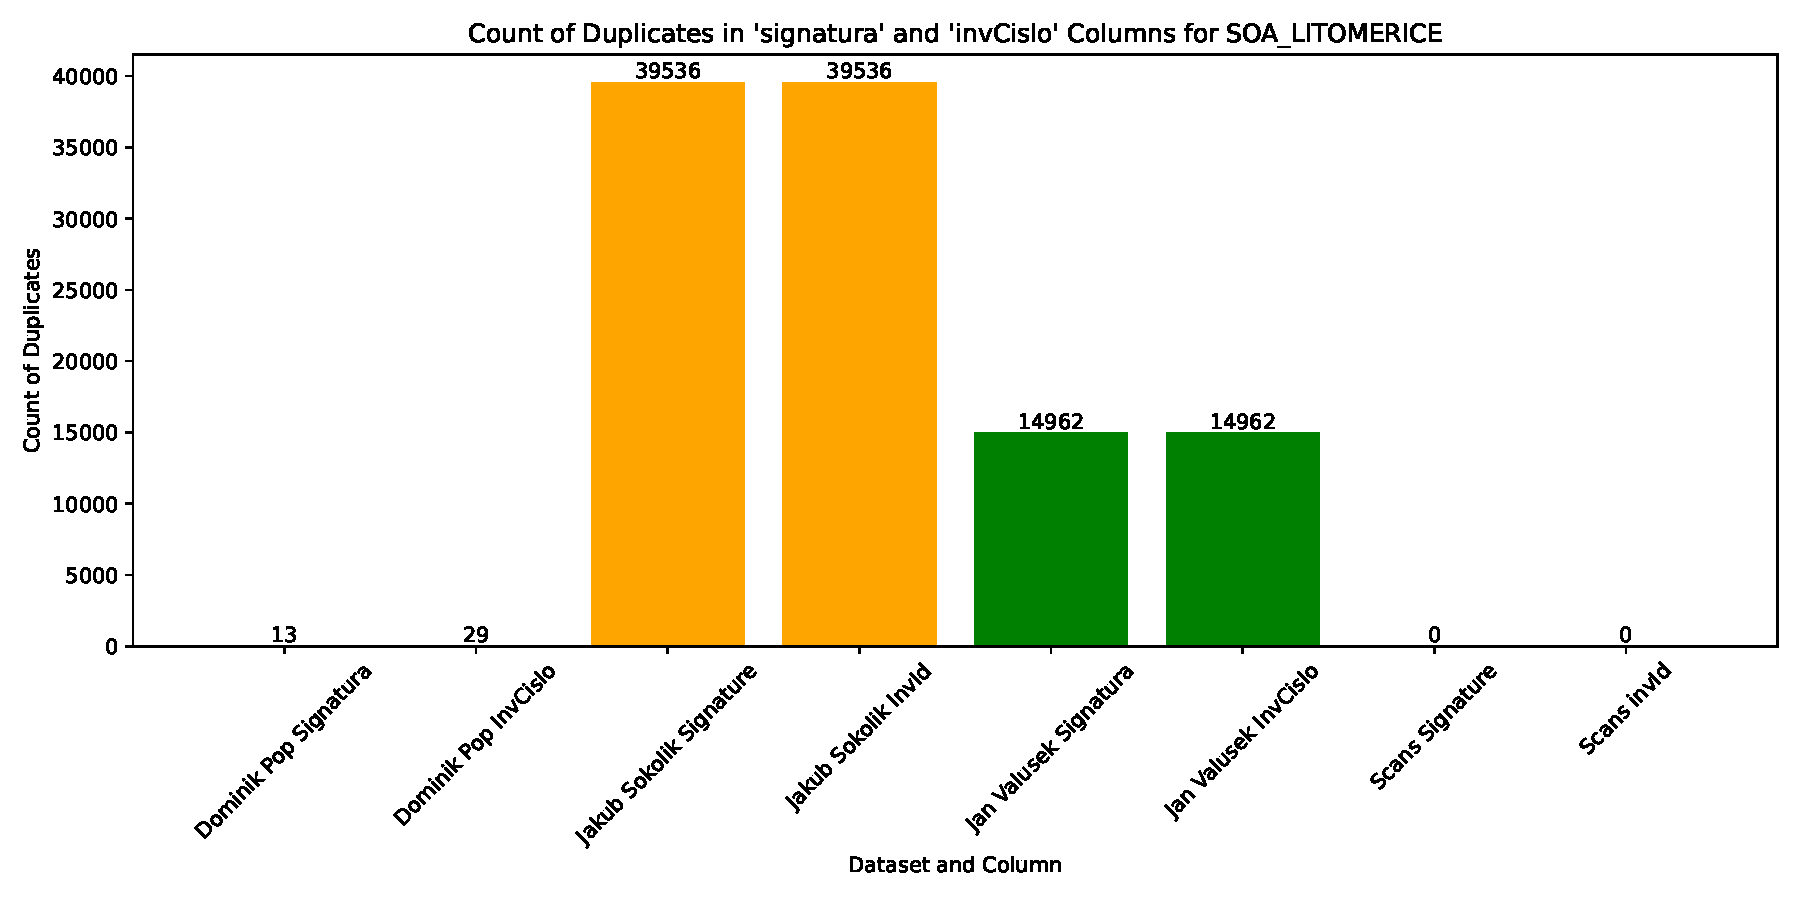
\includegraphics[scale=.5]{obrazky-figures/dataAnalysis/soaLitomerice/duplicities.pdf}
    \caption{Analýza duplicit pro SOA v Litoměřicích}
\end{figure}

\begin{figure}[htbp]
\centering
    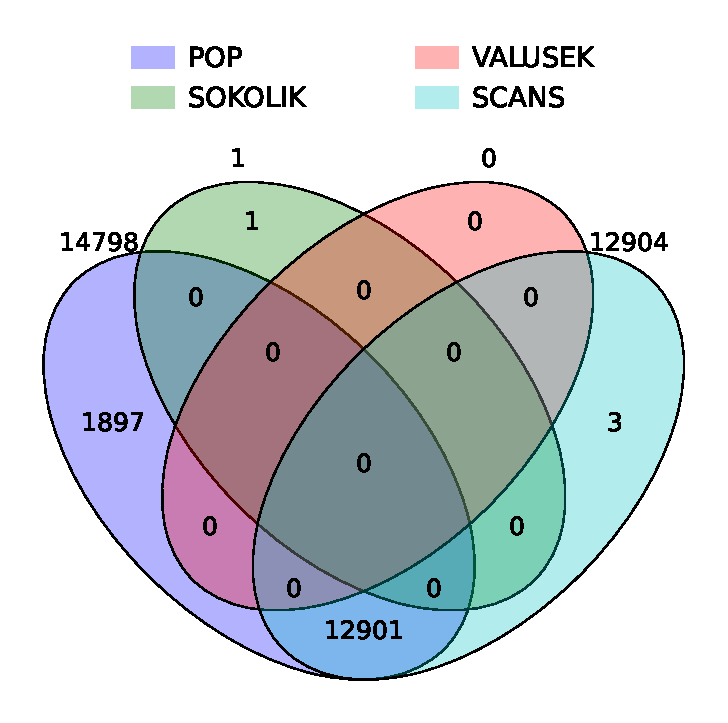
\includegraphics[scale=.5]{obrazky-figures/dataAnalysis/soaLitomerice/Venn_4.pdf}
    \caption{Vennuv diagram pro SOA v Litoměřicích}
\end{figure}


\newpage
\noindent\textbf{Zemský archiv v Opavě}\\

\begin{figure}[htbp]
\centering
    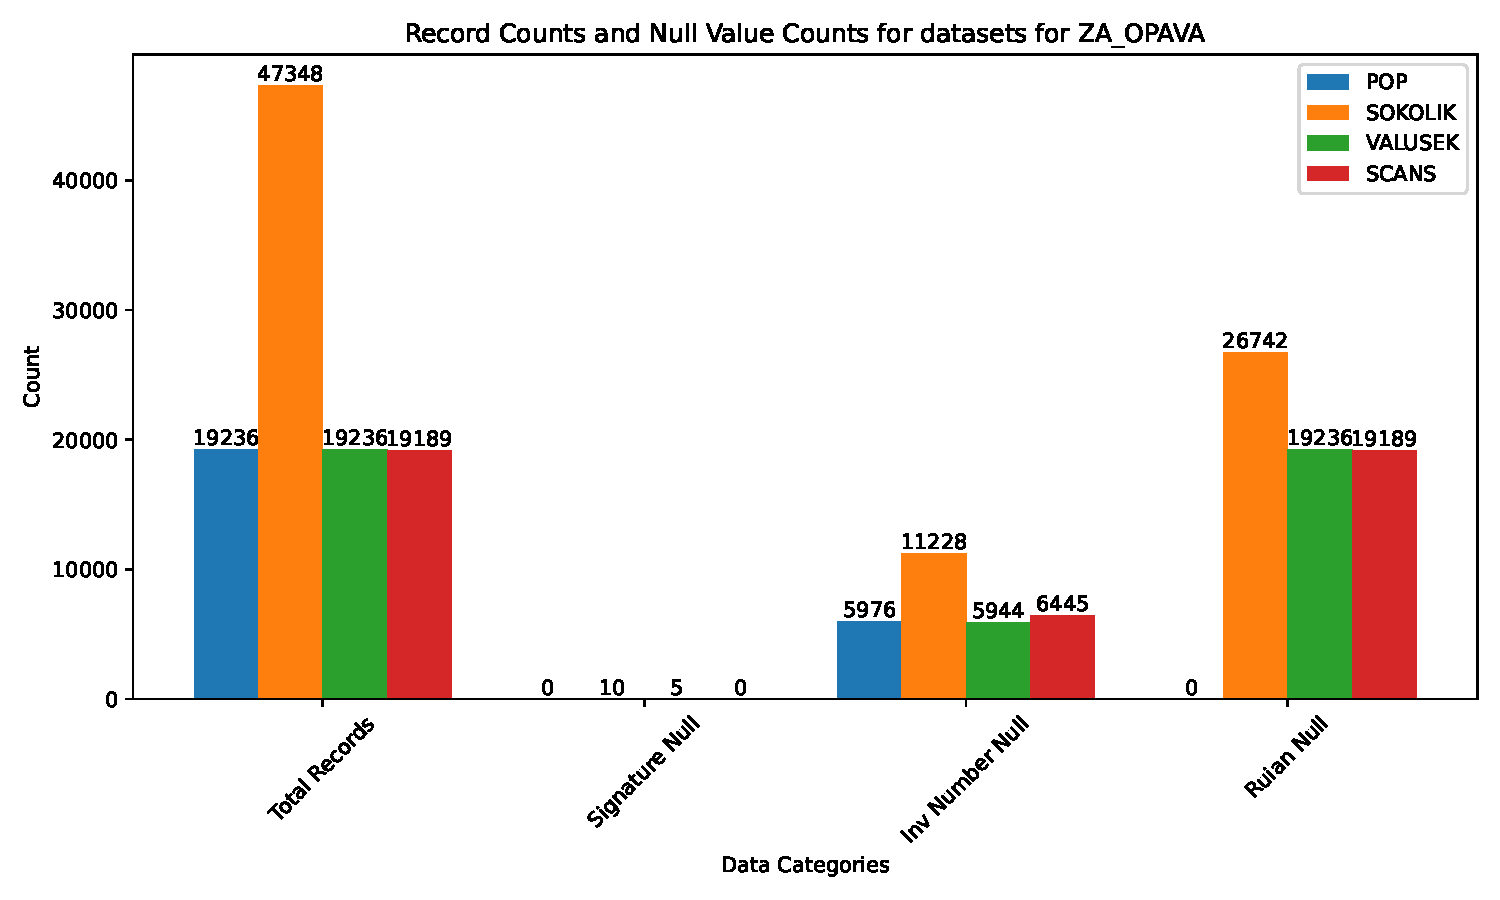
\includegraphics[scale=.5]{obrazky-figures/dataAnalysis/zaOpava/missingValues.pdf}
    \caption{Analýza chybějících hodnot pro ZA v Opavě}
\end{figure}

\begin{figure}[htbp]
\centering
    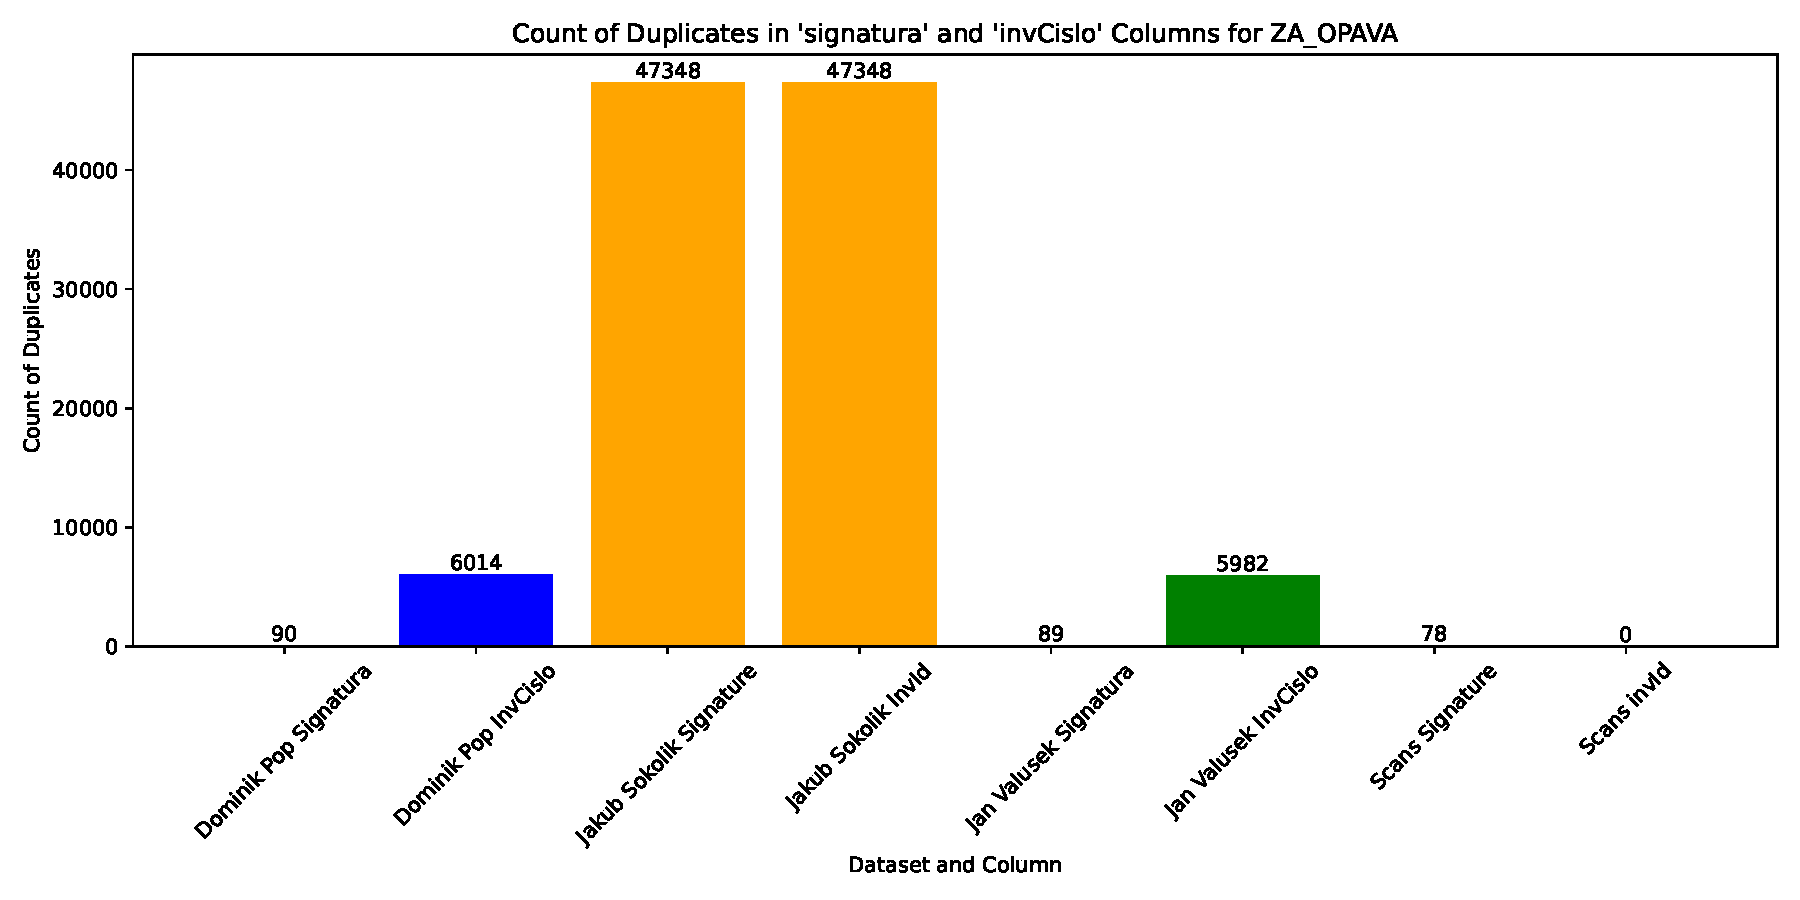
\includegraphics[scale=.5]{obrazky-figures/dataAnalysis/zaOpava/duplicities.pdf}
    \caption{Analýza duplicit pro ZA v Opavě}
\end{figure}

\begin{figure}[htbp]
\centering
    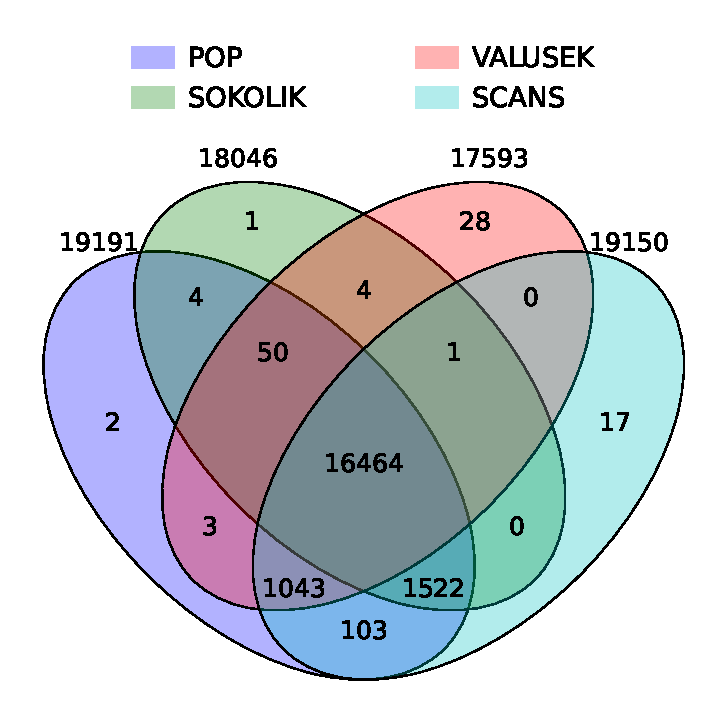
\includegraphics[scale=.5]{obrazky-figures/dataAnalysis/zaOpava/Venn_4.pdf}
    \caption{Vennuv diagram pro ZA v Opavě}
\end{figure}

\begin{figure}[htbp]
\centering
    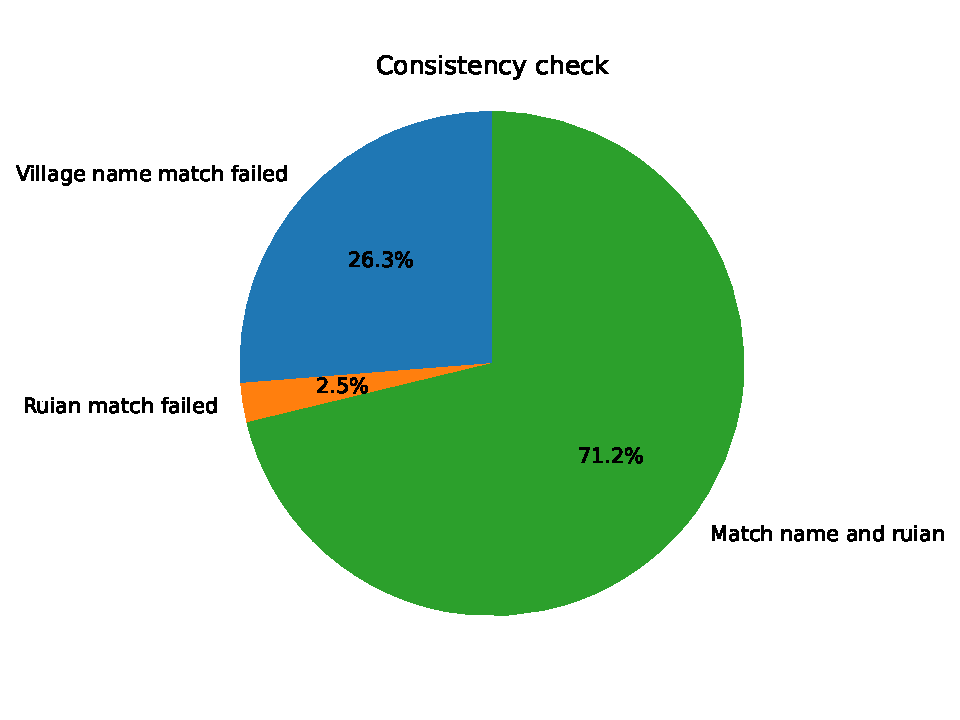
\includegraphics[scale=.5]{obrazky-figures/dataAnalysis/zaOpava/consistencyCheck2.pdf}
    \caption{Kontrola konzistence pro ZA v Opavě}
\end{figure}

\newpage
\noindent\textbf{Státní oblastní archiv v Plzni}\\

\begin{figure}[htbp]
\centering
    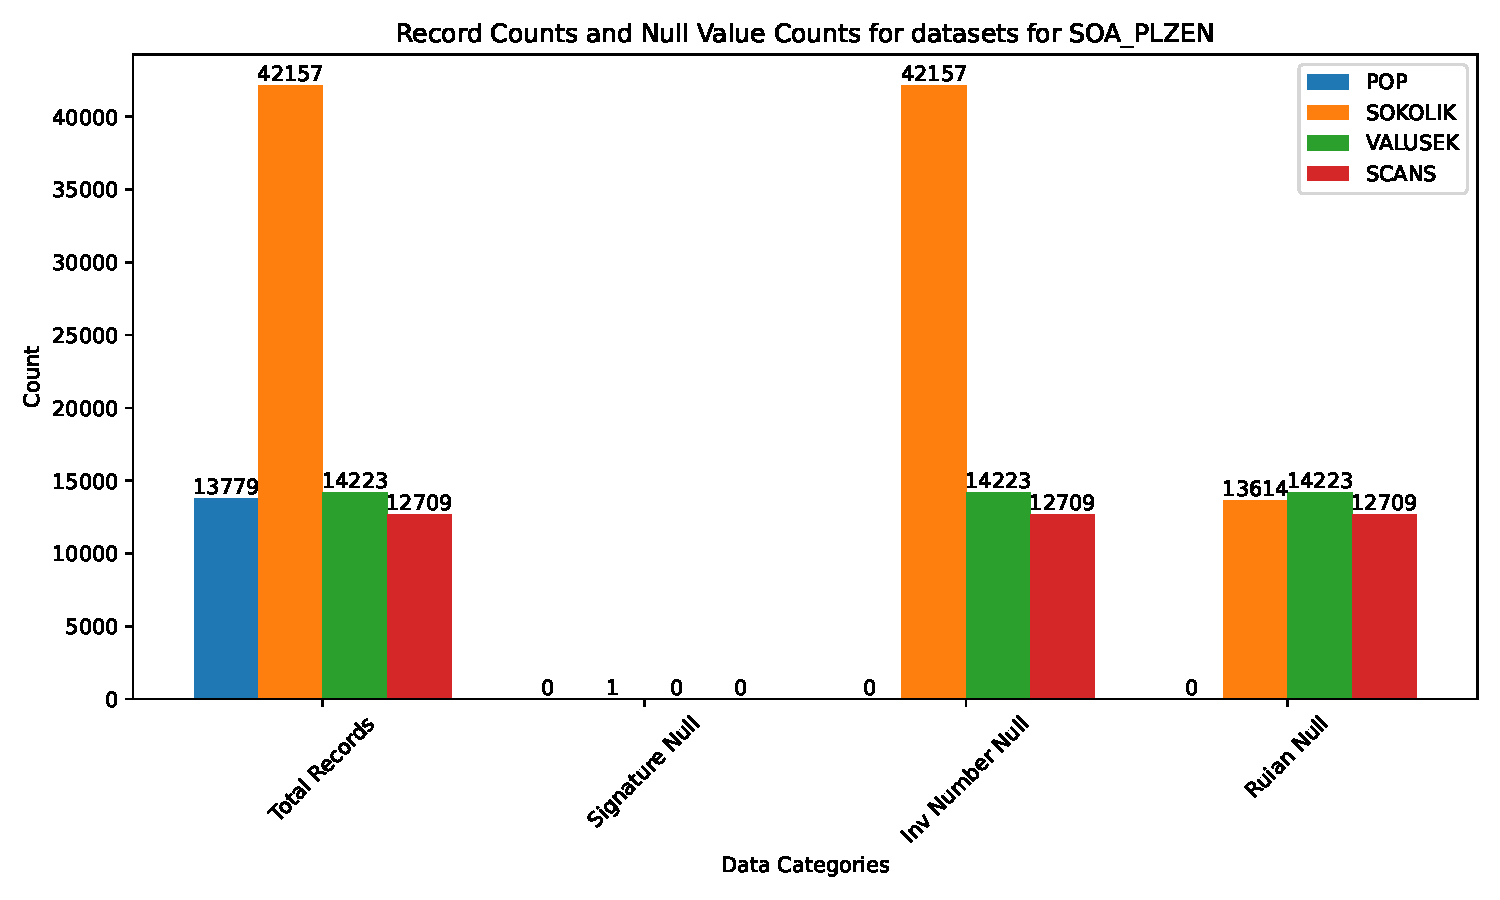
\includegraphics[scale=.5]{obrazky-figures/dataAnalysis/soaPlzen/missingValues.pdf}
    \caption{Analýza chybějících hodnot pro SOA v Plzni}
\end{figure}

\begin{figure}[htbp]
\centering
    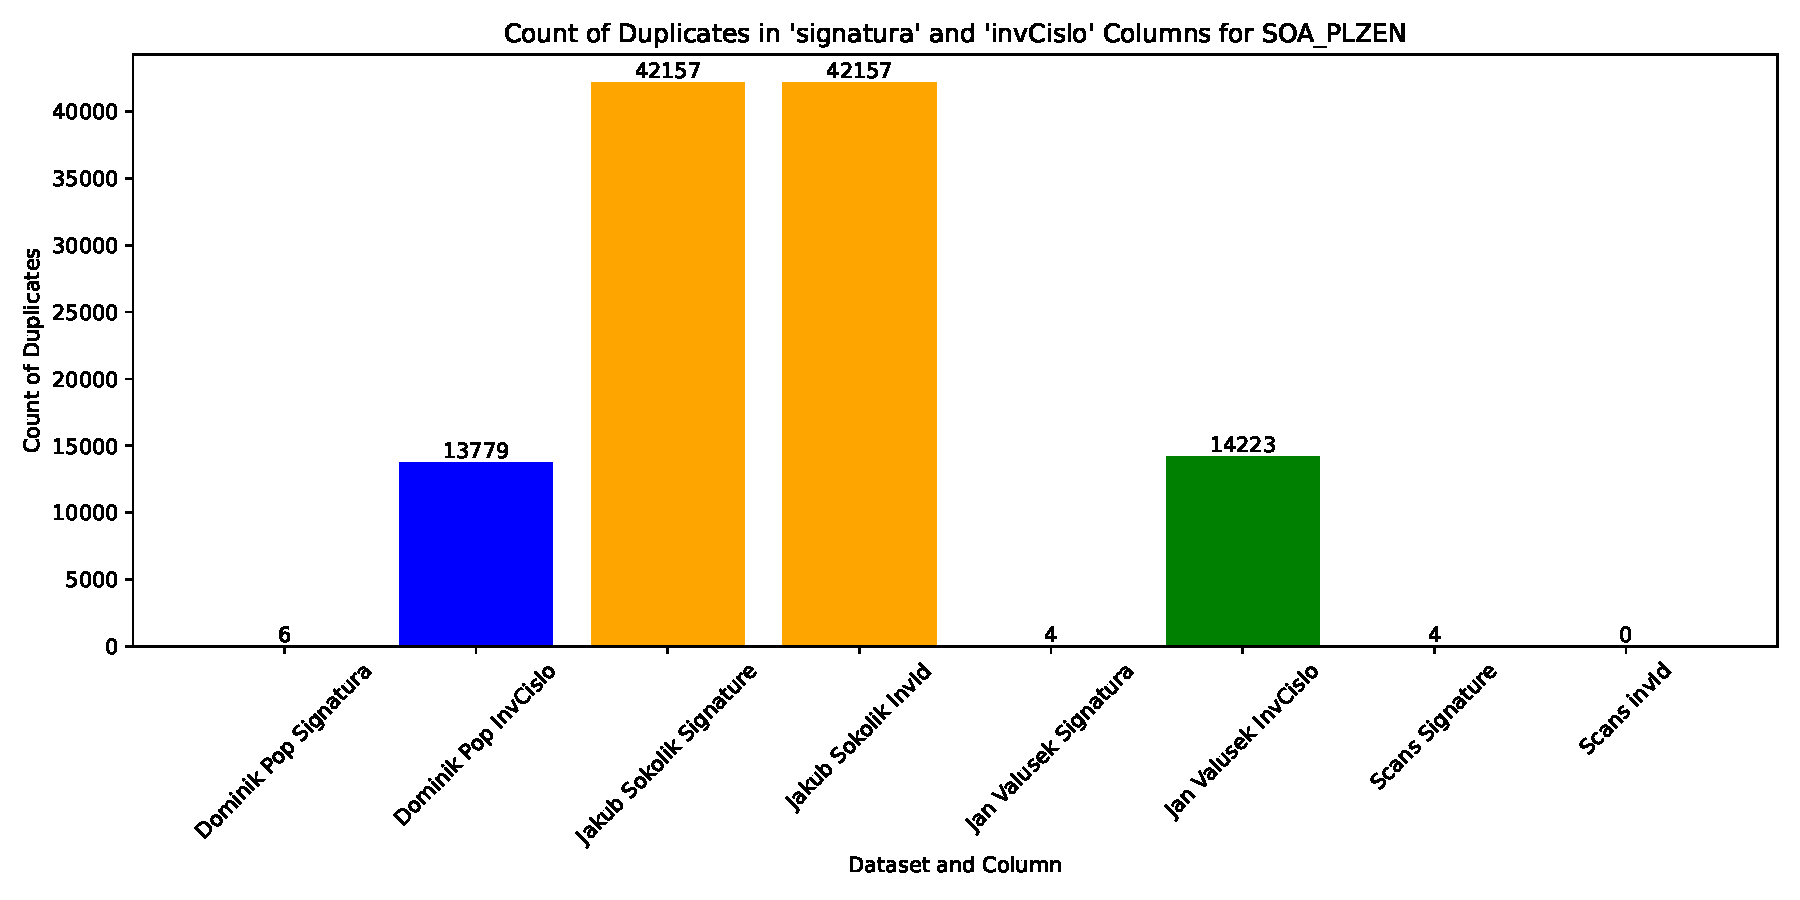
\includegraphics[scale=.5]{obrazky-figures/dataAnalysis/soaPlzen/duplicities.pdf}
    \caption{Analýza duplicit pro SOA v Plzni}
\end{figure}

\begin{figure}[htbp]
\centering
    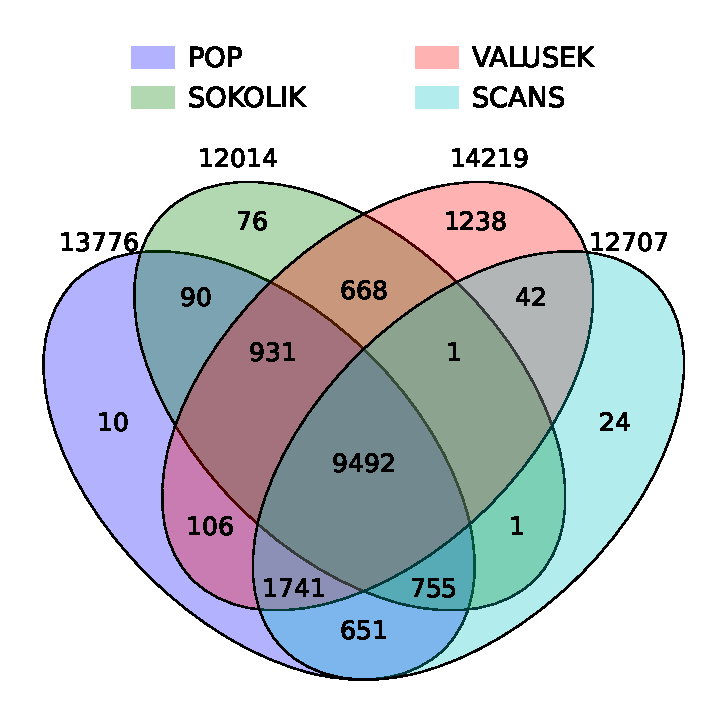
\includegraphics[scale=.5]{obrazky-figures/dataAnalysis/soaPlzen/Venn_4.pdf}
    \caption{Vennuv diagram pro SOA v Plzni}
\end{figure}

\begin{figure}[htbp]
\centering
    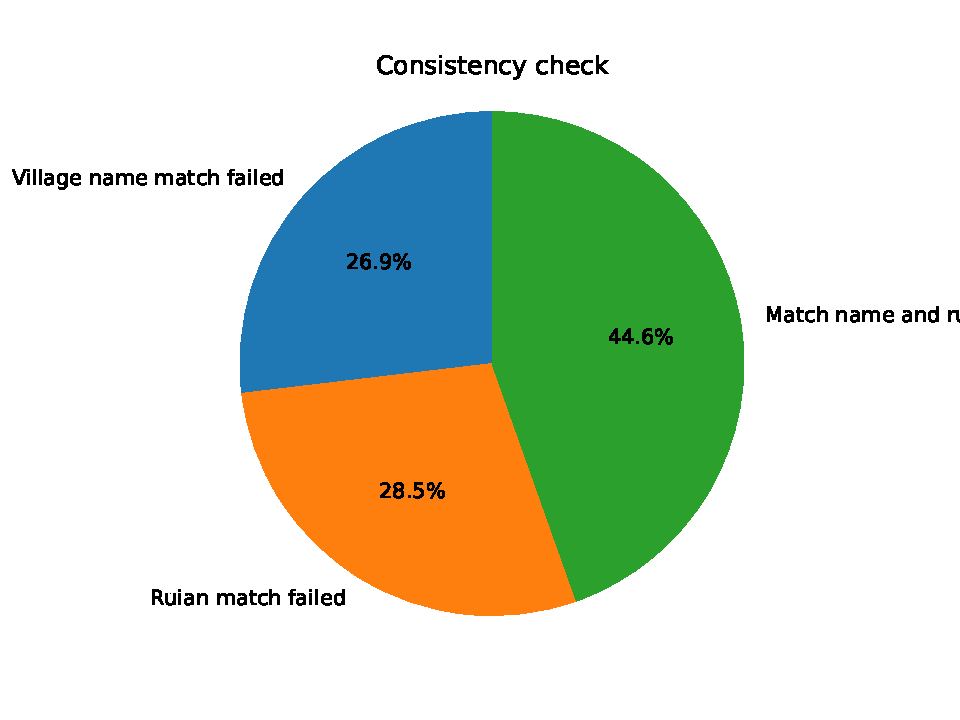
\includegraphics[scale=.5]{obrazky-figures/dataAnalysis/soaPlzen/consistencyCheck2.pdf}
    \caption{Kontrola konzistence pro SOA v Plzni}
\end{figure}


\newpage
\noindent\textbf{Státní oblastní archiv v Praze}\\

\begin{figure}[htbp]
\centering
    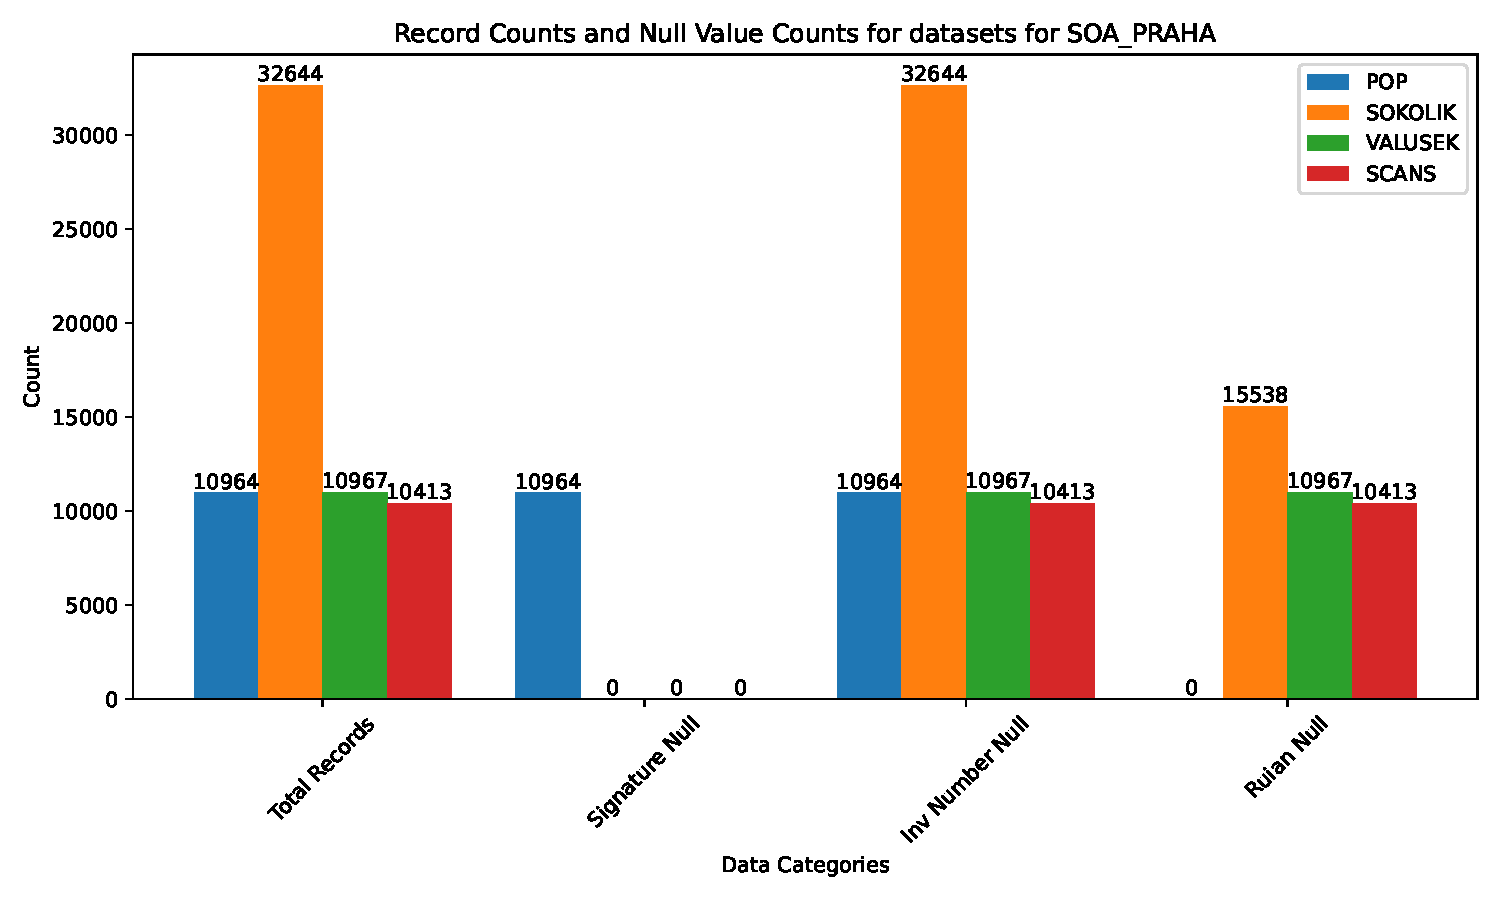
\includegraphics[scale=.5]{obrazky-figures/dataAnalysis/soaPraha/missingValues.pdf}
    \caption{Analýza chybějících hodnot pro SOA v Praze}
\end{figure}

\begin{figure}[htbp]
\centering
    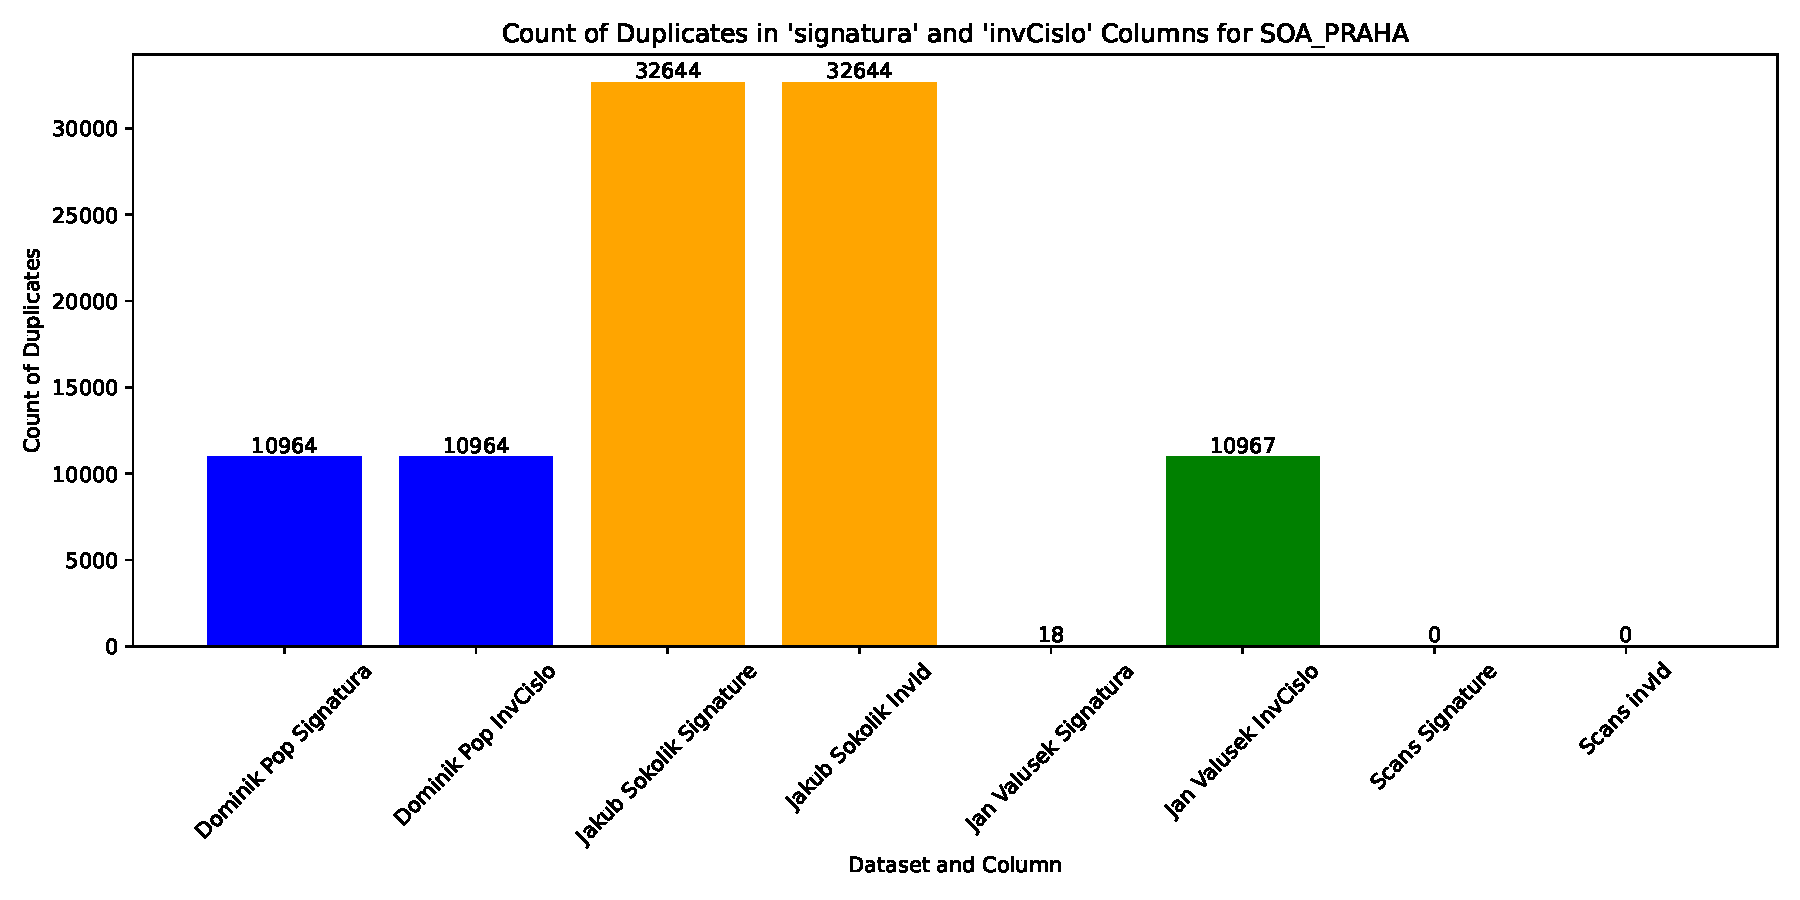
\includegraphics[scale=.5]{obrazky-figures/dataAnalysis/soaPraha/duplicities.pdf}
    \caption{Analýza duplicit pro SOA v Praze}
\end{figure}

\begin{figure}[htbp]
\centering
    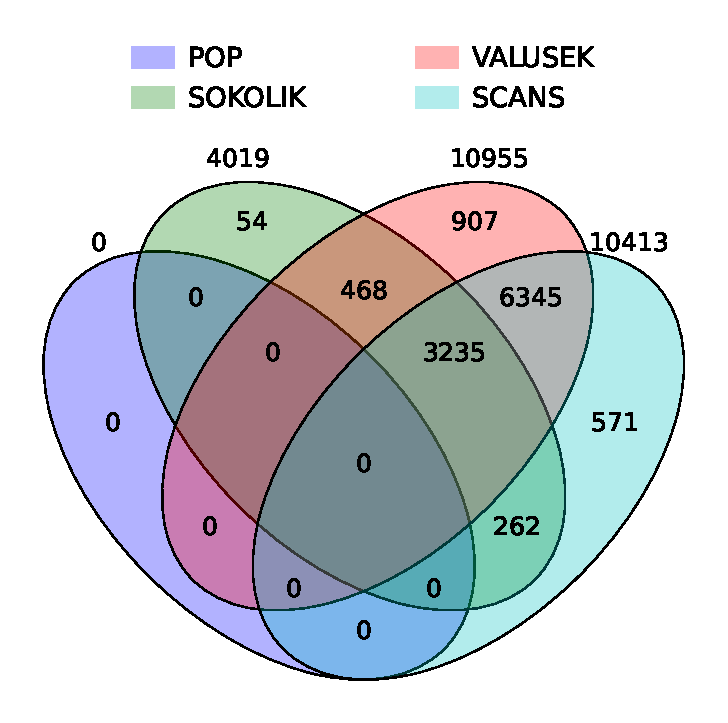
\includegraphics[scale=.5]{obrazky-figures/dataAnalysis/soaPraha/Venn_4.pdf}
    \caption{Vennuv diagram pro SOA v Praze}
\end{figure}


\newpage
\noindent\textbf{Státní oblastní archiv v Třeboni}\\

\begin{figure}[htbp]
\centering
    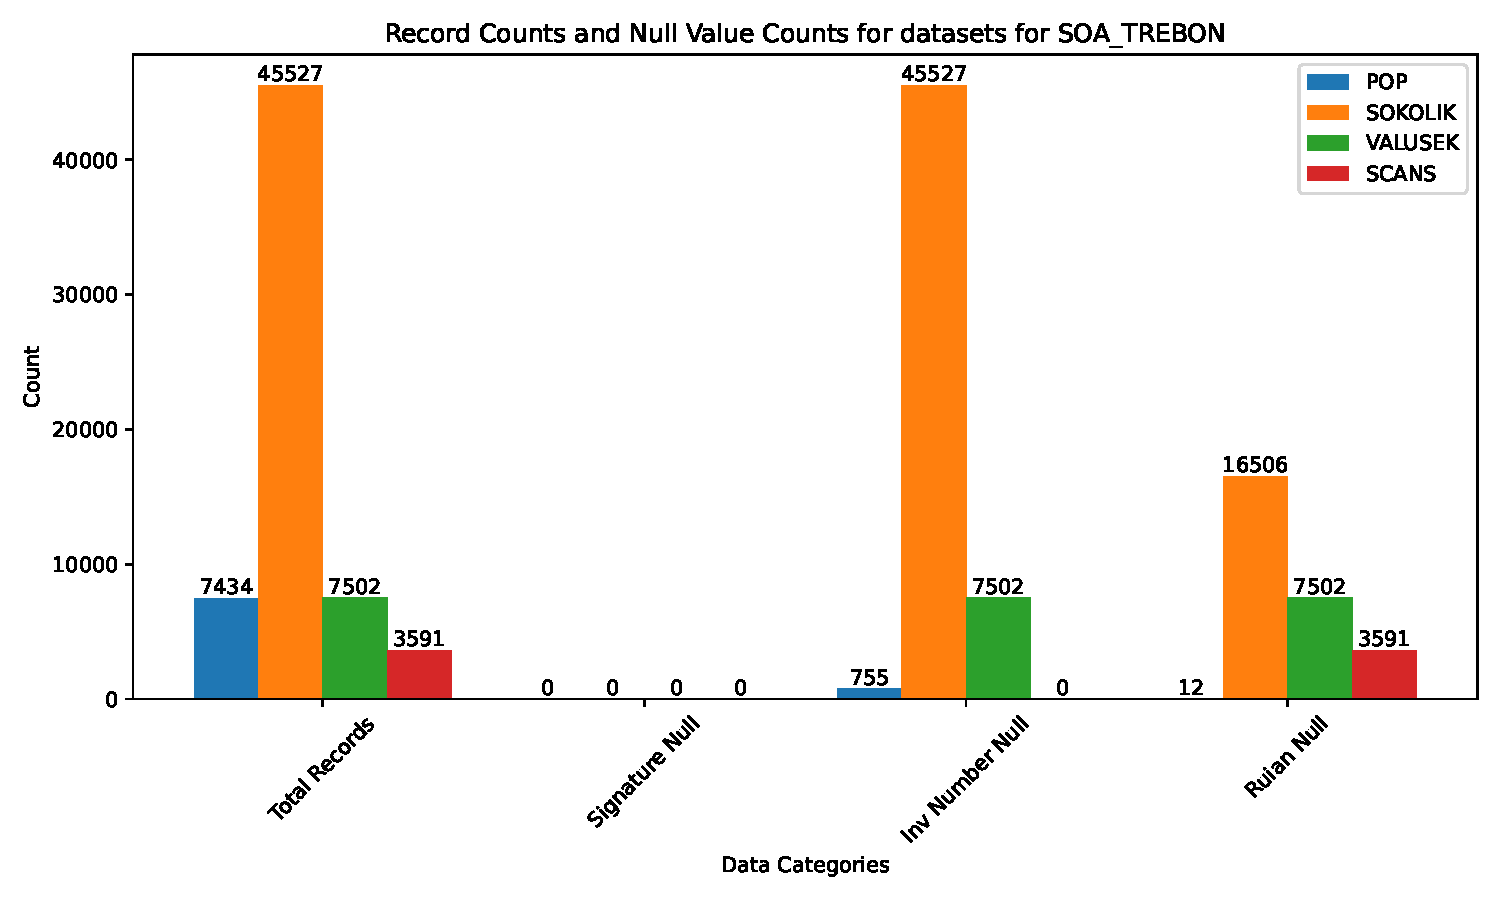
\includegraphics[scale=.5]{obrazky-figures/dataAnalysis/soaTrebon/missingValues.pdf}
    \caption{Analýza chybějících hodnot pro SOA v Třeboni}
\end{figure}

\begin{figure}[htbp]
\centering
    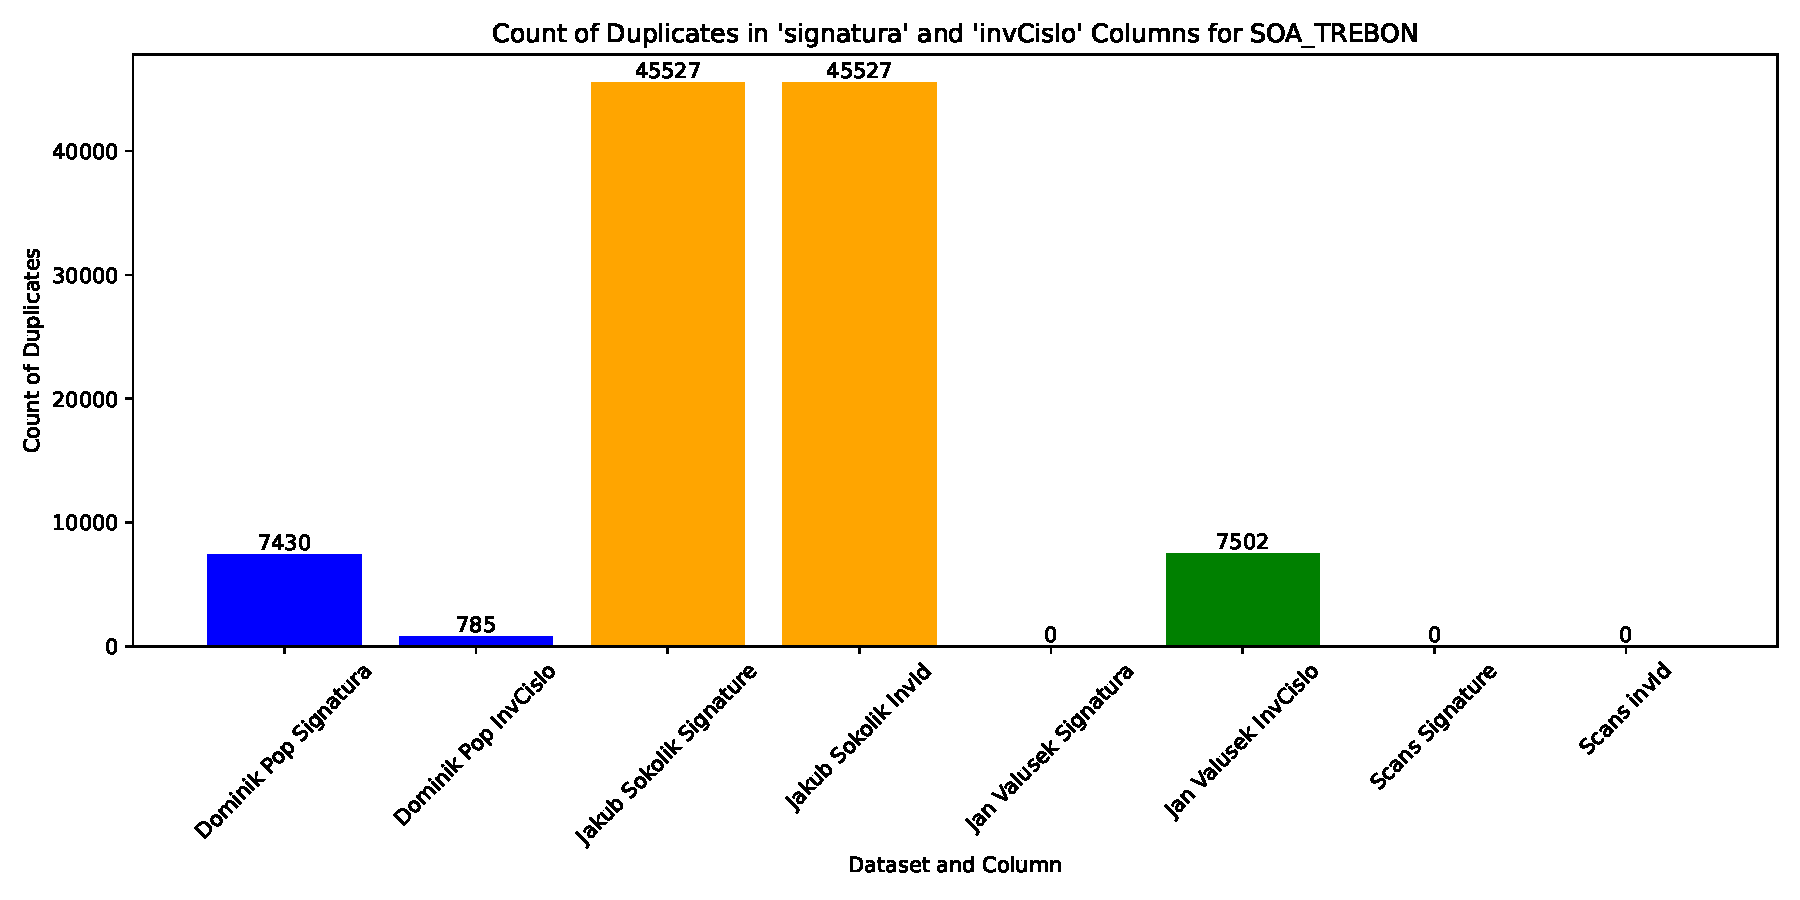
\includegraphics[scale=.5]{obrazky-figures/dataAnalysis/soaTrebon/duplicities.pdf}
    \caption{Analýza duplicit pro SOA v Třeboni}
\end{figure}

\begin{figure}[htbp]
\centering
    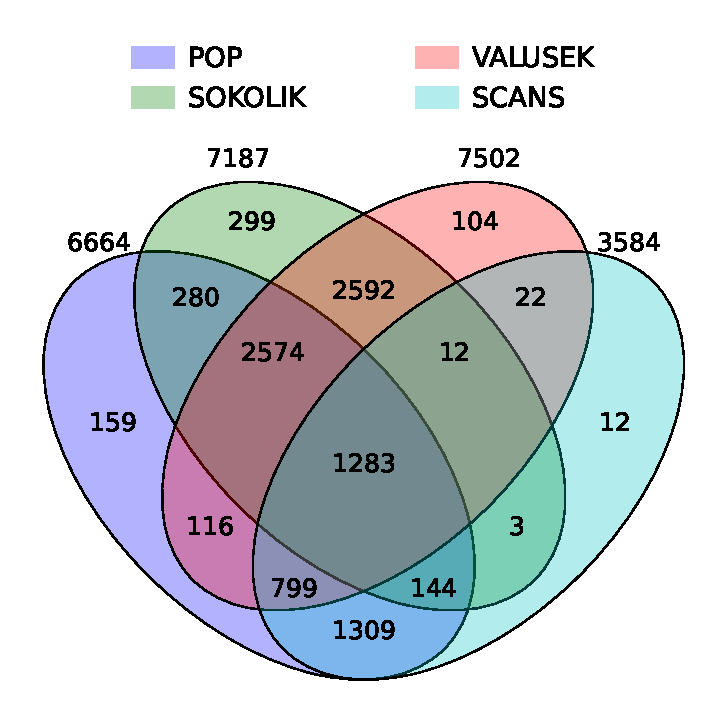
\includegraphics[scale=.5]{obrazky-figures/dataAnalysis/soaTrebon/Venn_4.pdf}
    \caption{Vennuv diagram pro SOA v Třeboni}
\end{figure}

